\documentclass[12pt, legalpaper]{article}
\usepackage{graphicx}
\usepackage{wrapfig}
\title{Rapport du projet Othello}
\author{FRENZEL Loïc\\HENRY Romaric}
\date{3 Juin 2025}
\renewcommand*\contentsname{Table des matières}


\begin{document}
\maketitle

\newpage

\tableofcontents

\newpage

\section{Introduction}

Le projet Othello a pour but de créer une IA\footnote{Ici le terme IA fait référence au IA 
des années 70-80 des algorithme, qui sont en faite des algorithme qui ont une recherche intéligente}
plus ou moins simple, selon les algorithme utilisé. Il fallait donc codé le jeu dans un premier temps
pour ensuite permettre de choisir parmis plusieurs mode de jeu :   
\begin{itemize}
    \item Joueur contre Joueur
    \item Joueur contre IA
    \item IA contre IA
\end{itemize}


Le partie devait originellement s'éxécuté sur terminal. Nous avons fais le chois d'ajouter une interface
graphique pour d'une certaine manière rendre le projet plus agréable et permettre de vaguement simplifié 
les changements de 
tour\footnote{Il s'avairera que dans le futur ce ne fut pas le choix le plus judicieuxdu moins aussi tôt dans le projet}.

Plusieurs algorithmes devait ensuite être implémenter pour l'IA avec différentes évaluations. 
Nous n'avons pas eu le temps de tout faire, nous nous sommes donc arrêté à l'élagage $\alpha$$\beta$.
La raison sera vue en détail dans la suite du document.

\newpage

\section{Les bases du jeu, l'architecture}
\subsection{Les premier pas}
Comme dit dans l'introduction au début du projet nous avons commencé sur une architecture simple 
qui éxécuté le jeu sur terminal (Cf le diagramme de classe)
\begin{figure}[h]
    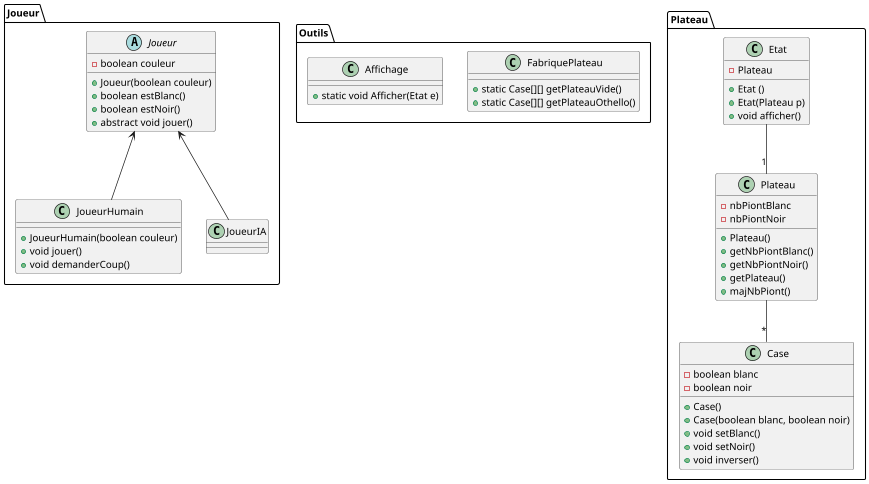
\includegraphics[scale=0.55]{othello}
    \caption{Premier diagramme de classe}
\end{figure}


Donc cette première architecture fut les bases de notre projet. Une des premières et denières
fois qu'on a bien réfléchis avant de codé.

Elle décompose bien les différentes classe du modèle.
Le package Joueur gère les joueur avec une classe abstraite pour pouvoir faire jouer sans
connaitre le type du joueur entre humain et le joueur IA.

Le package outil possède la classe Affichage et la classe FabriquePlateau.
La classe Affichage gère tous ce qui est relatif à l'affichage dans le terminal.
La classe FabriquePlateau permet d'obtenir le plateau initial mais aussi différents plateau
pour les tests.

Le package Plateau gère la plus grosse partie du modèle. Avec les classes Etat, Plateau et Case.
La classe Etat connait deux Joueur, qu'importe leur type réel. Elle sait aussi qui est le joueur
courant parmis les deux. Elle gère aussi tous ce qui est successeur d'elle même. Elle connait également
un plateau. La classe Plateau est là ou est décrit le plateau de jeu, elle connait le nombre de
piont blanc et noir, et une collection à deux dimensions de Case.
La classe case possède deux booléen : blanc et noir. Si les deux à false, la case est vide.
Si true à l'un ou l'autre ça veut dire qu'il y a un pion à cette endroit. Le fait que ce soit des
booléen facilite l'inversion des pion.

\subsection{Le début des problèmes}

Une classe Jeu piloté le tout et lancé une partie.
Mais très vite l'architecture des joueurs perdu sons sens puisque toute les fonctionnalité
du joueur humain furent mise dans la classe jeu. Cela posé beaucoup de problème d'évolutivité du code
mais aussi de compréhension et de conception. Ce problème resta longtemps dans le projet. 
Le changement ne sera opéré qu'une fois des bugs majeur sur le déroulé de la partie apparurent.
\\\par
Très vite après les premières partie lancé, nous avons décider de changer la structure du
projet pour ajouter une interface graphique. Cela nous à permis de mettre en pratique ce
qui à était vue dans une autre UE. Mais également de permettre dans une moindre mesure
simplifié le jeu à deux joueurs.
Son impact à était minimisé due à la présence du problème architectural précédement 
mis en exergue.
\\\par
Le modèle utilisé ici pour l'interface graphique est le modèle MVC. Il consiste en
une ou plusieurs classe qui sont les sujet observé qui vont rafraichir les observateurs,
les vue à chacune de leur modification. Mais la relation est dans les deux sens, puisque
les controlleurs peuvent détecter des actions de l'utilisateurs et ensuite demandé
appliqué des modification sur le sujet observé.

\begin{figure}[h]
    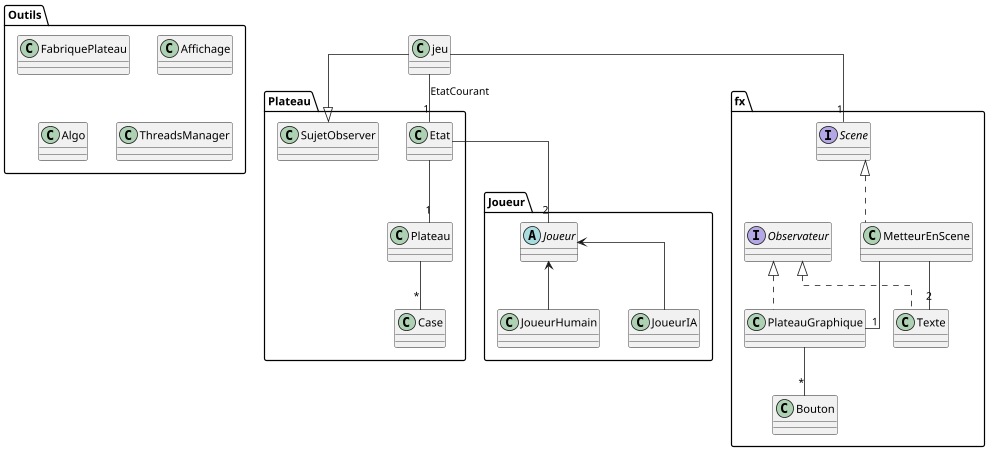
\includegraphics[scale=0.5]{othello2}
    \caption{Deuxième diagramme de classe}
\end{figure}

Ici le sujet observé fut donc la classe Jeu, et l'observateur fut la classe PlateauGraphique.
La classe PlateauGraphique est composé d'une grille constitué de bouton.
Si le bouton était cliqué une demande de coup était demandé au jeu, cela ne ce faisait
que si le joueur courant était un joueur humain. Si le coup était valide, le bouton
affiche une image de pion selon la couleur du joueur courant. Sinon une exception est
affiché à l'écran, informant que le coup est invalide.

\subsection{Des IA et des problèmes}
Des problèmes apparurent un peu plus tard quand le joueur IA fut jouable, puisque
le plateau graphique ne signalais pas le coup au joueur mais au jeu. Ce qui fait que
d'une part la classe joueur perd tout son sens, mais d'autre part qu'il n'y a presque
aucune logique de tour, hormis que dans le modèle on change d'état. Mais cela ne se 
faisait pas bien du à ce soucis de conception.

Pour rester dans ce problème de conception, l'entierté du programme du joueur IA
était également réalisé dans la classe jeu...
Il avait aussi des problèmes sur le fonctionnement même de l'IA mais cela sera abordé
dans une partie futur.

\subsection{Une solution...}
La décision fut prise de refactorisé le code, pour enfin respecter le principe de JAVA
mais aussi d'avoir quelque chose de clair. 
Les classes des joueurs eurent enfin une vrais utilité, leurs codes qui leur revenaient
de droit y furent implémantés.

L'interface graphique à chaque action du joueur sur le plateau, s'il est possible,
demande de jouer un coup au joueur courant.
Si ce n'est pas le tour d'un joueur humain, le platrau n'est pas réactif.
A chaque nouveau tour, le joueur courant regarde s'il a des coups possible, si oui il
attend pour le joueur humain, détermnine le meilleur coup pour l'IA. Si aucun coup
possible le joueur passe son tour, l'Etat et le joueur courant change.
\\\par
Malheuresement même après tous cela des bugs perssiste. Mais cela à lieux au niveaux du
joueur IA.

\subsection{Une complexité des IA}
Les IA avec une intarface graphique sont doté d'une petite spécifité. Puisque le calcul
du coup qu'elle va jouer est très demandant, elle va entièrement coupé toutes autres 
actions. Ce qui fait que le joueur humain va jouer un coup puis l'IA va faire le sien
après un certain temps, mais on aura pas vue le coup du joueur humain ce placer, due
au faite que l'interface fut bloqué puis rafraichis deux fois de suite.

Pour réglé ce problème il faut créer un thread dans le joueur IA qui va s'occuper
d'aouter un certain temps d'attente lorsque que la profondeur de recherche et très courte
puis de demandé à l'IA de chercher un coup. Il faut aussi ajouter une classe pour 
géré les thread et les tué une fois qu'ils sont inutiles.

\newpage


\section{Ajout de l'algorithme MinMax}
\subsection{Algorithme et évaluation}
\subsection{Refactorisation du code}
\subsection{Les problèmes contre-attaques}
\subsection{piste de solution}

\newpage

\section{algorithme avec élagage $\alpha$ $\beta$ }

\newpage

\section{Une suite ...}
Raison pas plus ...
Assez bref je pense


\section{Conclusion}
problème conception $->$ raison + leçon tiré



\end{document}